In this chapter, we will now extend our study on composite resonator systems. Such that, we will increase the number of resonators in our system. These structures, that will be discussed here, were not optimized to acheive enhanced dispersion. Rather the purpose of these analysis is to demonstrate the versatility of cascaded resonances. For the scope of this thesis, the resonators will be again ring shaped resonators and thus we will study properties of such ring resonators and study their mutual coupling effects.
\section{Triple Resonator System}
Now we are going to introduce a new geometery, basically what we are going to do is add another ring above the coupled two resonator system which were discussed before in chapter 3. Now we have a three resonator system with each have their own distinct resonant frequencies. Fig 4.1 displays the basic geometery.

These resonators show distinct properties due to introduction of another ring with a higher Quality-factor, coupled to the two resonator system. This will allow us to observe multiple resonances and observe phenomenons like CRIT and CRIA with another perspective. This will also enable us to simultaneously measure these effects in a single system and thus obtain transmission and dispersion of useful product.


The diagram shows us that the three rings are mutually coupled to the optical waveguide and thus the energy from the input is labled as $E_{1}$ which couples the resonator 1 due to evanescent coupling and the energy transfer is then $E_{3}$. This energy travels the first ring and is again coupled into the resonator 2 as $E_{5}$ and then again into the resonator 3 with energy $E_{7}$. Then it loops back into the waveguide as $E_{8}$, $E_{6}$ and $E_{4}$ respectively to couple back to the waveguide, each acquiring a distinct phase shift and outputs the signal with $E_{2}$.

\begin{figure}[h]
\centering
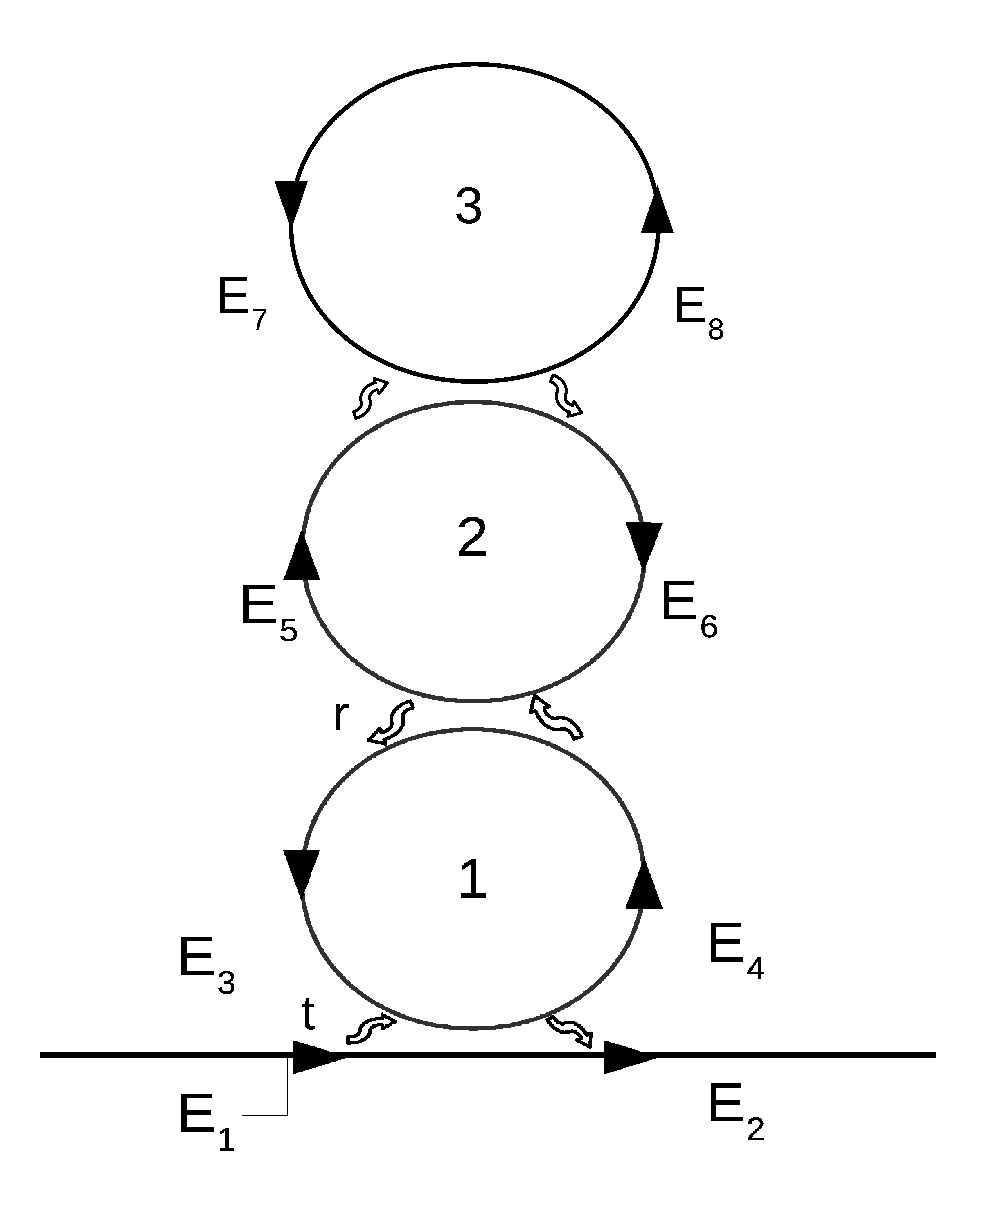
\includegraphics[scale=0.45]{triple_ring_resonator.eps}
\caption{Basic illustration of three ring resonator geometery along with its respective fields.}
\end{figure}

\subsection{Transmission and Phase relations}
The complex transmitivity and its respective phase can be determine by the equation 4.1 and 4.2 respectively. 

\begin{equation}
\frac{E_{t}}{E_{i}} = \frac{r_{1} - a_{1} r_{12} e^{i\phi_{1}}}{1 - r_{1} r_{12} a_{1} e^{i\phi_{1}}}
\end{equation}

where, 
\begin{center}

$r_{12} = \frac{r_{2} - a_{2} r_{23} e^{i \phi_{2}}} {1 - r_{2} r_{23} a_{2} e^{i \phi_{2}}} $
and,
$r_{23} = \frac{r_{3} - a_{3} e^{i \phi_{3}}} {1 - r_{3} a_{3} e^{i \phi_{3}}} $

\end{center}

Similarly, the effective phase of the complex transmitivity is given by:

\begin{equation}
\phi_{eff} = \arctan[{\frac{r_{1} |r_{12}| a_{1} \sin{(\phi_{1} + \phi_{12})}}{1 - |r_{12}| a_{1} \cos{(\phi_{1} + \phi_{12})}}}] - \arctan[{\frac{|r_{12}| a_{1} \sin{(\phi_{1} + \phi_{12})}}{r_{1} - |r_{12}| a_{1} \cos{(\phi_{1} + \phi_{12})}}}]
\end{equation}

Now we will try to model these equations to observe different results.

\subsection{Passive three resonances results}
We can obtain very interesting results from a passive three resonator systems some of which will be discussed in this section. Fig. 4.2 displays EIT inside an EIA transmission with negative group index and fast light. These cascaded resonances can help play an important role in the tunability of fast and slow light and/or in large and small absorption of resonant frequencies. This will generate new applications according to the needs. These kind of effects which were measured in atomic systems in which most of the light was absorbed, can now be acheived in these rather simple resonator systems. 

In figure 4.2, we see that the transmission spectrum looks like an CRIA dip, meaning it will display the properties of CRIA. When we zoom into the graph (as shown on the right), we observe that there is another peak rising within the CRIA, showing the resonance of the resonator 3. Thus now we have CRIT inside a CRIA transmission. This will allow us to have maximum transmission intensity on the other side with properties of CRIA. Meaning now we can have more light in coupled resonator induced absorption.

The effective phase of the system is shown in red where we see a normal curve stretching from positive to negative x and y axis. But when we zoom into the middle of the curve, we see two resonances displaying the effects of the coupled three resonantors. The zoomed version is shown on the right in fig. 4.2 and it displays negative slope on resonance meaning the light we are receiving from the EIT transmission is fast light. Thus we can say that we have superluminal light from a maximum EIT transmission with EIA like properties.

\begin{figure}[h]
\centering
\includegraphics[width=1\textwidth]{EIT_EIA_all.eps}
\caption{EIT observered in an EIA transmission in three resonator system with its phase in red and group index in green.}
\end{figure}


Now we will observe that the transmission can be a lot influenced if we were to change the coupling effects between the resonators. This tells us a lot about how our signal is transmitted and how much use can we acheive from the single system by changing a bit of its properties. In figure 4.3, we change the coupling parameters in all of the resonators and have acheived a rather intresting transmission spectrum. We can clearly see what looks like an absorption spectrum of a single resonator, has a narrow peak of EIT like transmission within it (zoomed on the right). This peak also has a dip on resonance due to the third coupling of the resonator. Now we have an interesting result of EIT within an absorption and EIA withing that EIT. 

\begin{figure}[h]
\centering
\includegraphics[width=1\textwidth]{EIT_EIA2_all.eps}
\caption{Cascaded resonance effects in three resonator system with its phase in red and group index in green.}
\end{figure}


The effective phase of the system, at first, also seems like that of an single resonator system but zooming into the graph tells another story. On the right, we can see three distinct resonances caused by the coupling of the three resonator system and we have negative slope on resonance. This negative slope tells us that we are getting superluminal light on the resonant frequencies. 

The group index plot, shown in green, also displays negative group index on resonance and positive index peaks off resonances. The negative group delay also predicts superluminal velocities of the resonant frequencies.

After these interesting results, let us now jump into another useful transmission spectrum of our triple resonator system. This spectrum is also acheived by the same arrangement of the resonators and now we have changed the coupling effects once more to obtain a beautiful result. 

\begin{figure}[h]
\centering
\includegraphics[width=1\textwidth]{EIAinEIT.eps}
\caption{EIA observered in an EIT transmission in three resonator system with its phase in red and group index in green.}
\end{figure}

In figure 4.4, we can see a specetrum which resembles the graph of an EIT transmission as in Coupled Resonator Induced Transmission. When we again zoom into the transmission, we see a narrow dip on resonance. This narrow dip shows us that we have an effect like CRIA in this resonance. 

We see that the graph dips to zero almost, meaning all of the light is absorbed. This transmission dip tell us that we can filter out exactly this narrow spectrum of resonant frequencies. 
The phase of the system is shown in red. we again see that the curve is simple but have sharp resonances this time of a quite high value, on resonance. The slope of this graph is almost zero on resonance.

The group index, shown in green, also displays group index very near to zero in this graph. Although its value is $\approx -0.37$ meaning superluminal velocities of resonant frequencies. But almost all of the resonant light is blocked/absorbed thus this value is practically useless.

\subsubsection{Double EIA}
After that we have seen and observed CRIT and CRIA effects withing each other, let us now see CRIA two times occuring in a single spectrum. This double EIA or CRIA is obtained by slight detuning of the system and changing the coupling effects. 

In fig. 4.5 we can clearly see that two narrow peaks, which are caused by the two resonances of the coupled resonators, 2 and 3 respectively. And the broader dip above them is caused by the resonance of the resonantor 1. 


This allowed us to observe an effect which resembles the CRIA in two resonator system but this time now we have two narrow dips off resonances.

This tells us that we have CRIA like properties and transmission have two narrow absorption lines but on the off-resonance. The resonant frequencies will experience very little absorption and will be mostly transmitted. 

The phase and group velocites of this case is not discussed as the purpose of these study was not to discuss the enhanced dispersion. The dispersive properties of these resonances will be similar to the ones discussed above. The true meaning is to show enhanced transmittance.

\begin{figure}[h]
\centering
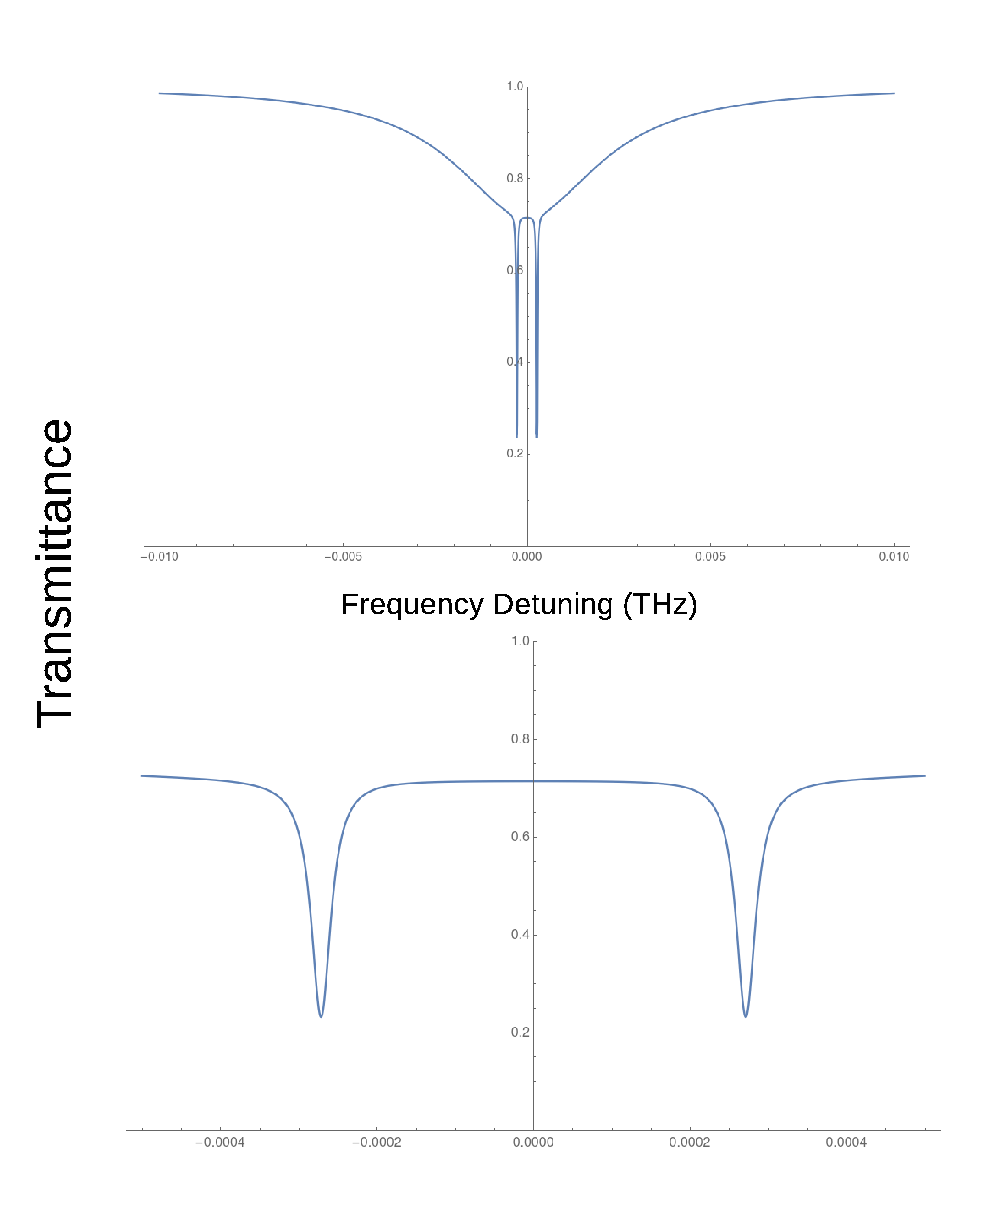
\includegraphics[scale=0.5]{double_EIA.eps}
\caption{Double absorption dips observed inside an EIA like transmission off resonant to the spectrum.}
\end{figure}

From these results, we concluded that increasing the number of resonators in the system and mutually coupling them with each other, enables us to demonstrate the versatility of the cascaded resonances. These resonances can be then utilized and acheived in practical applications to make use of them in important tasks. Optical tunability and signal filteration of specific frequencies can be acheived by using similar systems and having similar effects in them.
\newpage
